% -*- coding: utf-8 -*-
\documentclass{oblivoir}
\usepackage[utf8]{inputenc}
\usepackage{kotex}
\usepackage{graphicx}
\usepackage{subfig} % 한 줄에 여러 이미지 출력을 위함.
\usepackage{indentfirst} % 첫 문단의 indent를 Tab
\usepackage{amsmath} % 행렬
\usepackage[a4paper,left=30mm,right=30mm,top=40mm,bottom=30mm]{geometry}
\title{Graph Mining \large \\
	Graph에서 Frequent Subgraph를 찾는 법}
\author{201824633}

\begin{document}
	\maketitle
	\section {Graph Mining}
		\label{graph_mining}
		Data Mining은 데이터로부터 새로운 지식을 발견해내는 과정으로, 수많은 데이터의 산에서 가치있는 정보를 찾는다. 그 후 우연이 아닌 인과관계로부터 패턴을 찾아내서 추출한다. Data Mining에는 Text Mining, Association Rule Mining, Graph Mining 등의 다양한 분야가 존재한다. 그 중 Graph Mining은 활용도가 매우 높다.
		
		 
		 Graph Mining이란, 한 그래프에서 자주 사용되는 Subgraph들을 찾아내는 것이다. 이 때 그래프는 어느 분야에서든 다양한 형태로 존재한다. 그에 대한 예시는 그림 \ref {graphs}과 같다. 
		\begin{figure}[h]
			\centering
			\subfloat[Aspirin 구조]{{
					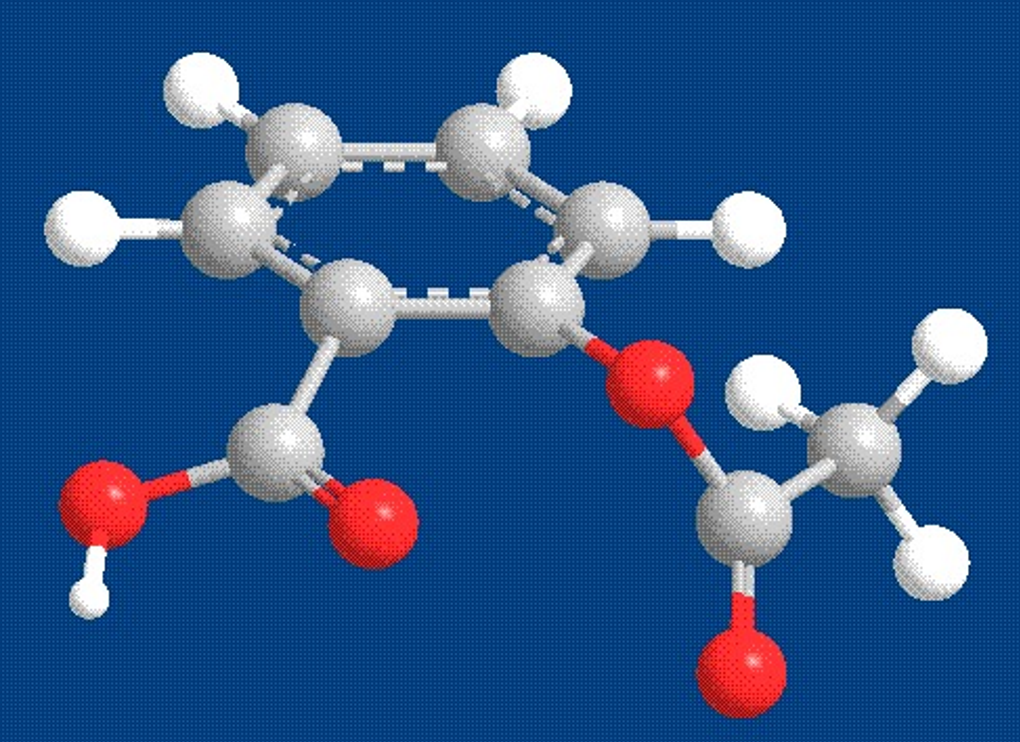
\includegraphics[width=.4\linewidth]{figure/aspirin}
					\label{aspirin}
			}}
			\quad % tab : quad 1번 qquad 2번 => 얘 없으면 안됨
			\subfloat[Co-Author]{{
					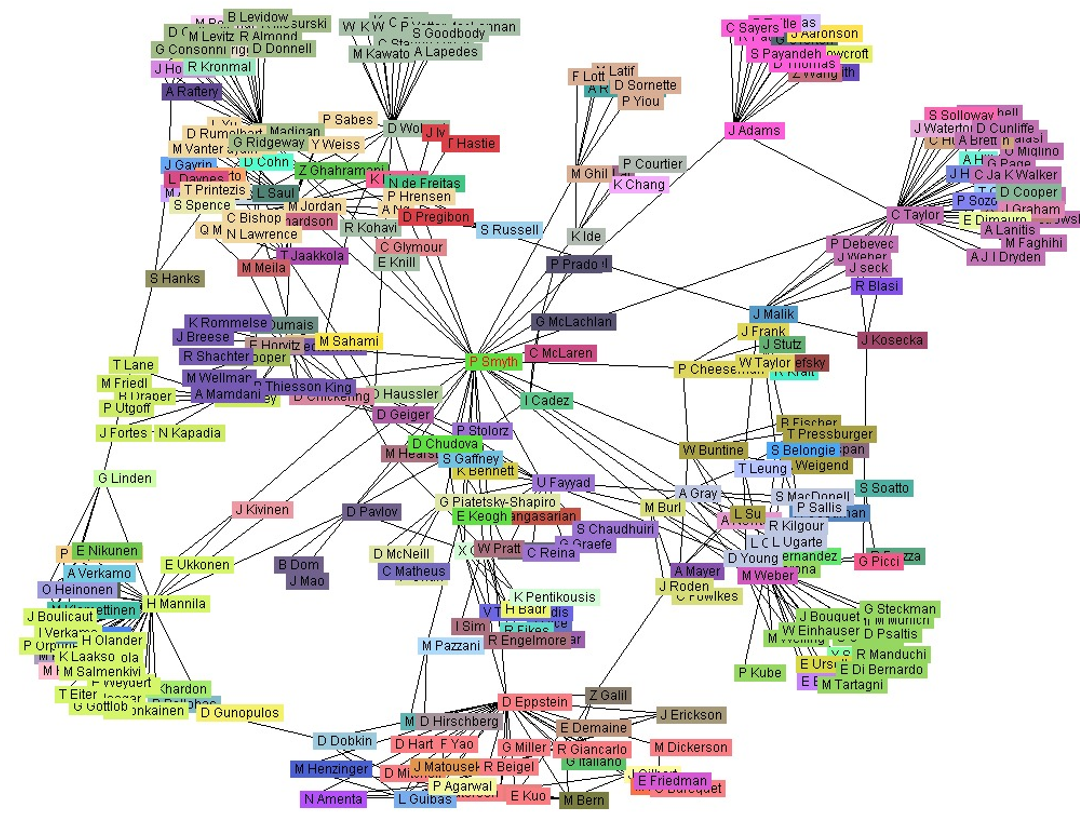
\includegraphics[width=.4\linewidth]{figure/co-author} 
					\label{co-author}	
			}}
			\caption{다양한 분야에서 사용되는 그래프들}
			\label{graphs}
		\end{figure}
		
		
		위의 그림 \ref {aspirin}은 신약 개발을 위한 기존 약의 단백질 구조, 그림 \ref{co-author}는 사람들간의 관계를 표시한 그래프이다.
	
	\section {Frequent Subgraph Approaches}
		\ref{graph_mining}절에서 Graph Mining이란 그래프에서 자주 사용되는 Subgraph들을 찾아내는 것이라고 했다.  Subgraph를 찾아내는 방법에 대해 알아보자.
		
		\subsection{Apriori-based approach}
		Apriori-like Algorithm은 vertex 또는 edge를 하나씩 늘려가며 조건에 맞는 subgraph를 다음 단계로 진행시키는 방식이다. 상세 방법은 다음과 같다.
		
		\begin{enumerate}
			\item 1-subgraph를 찾는다. \label{apriori1}
			\item Candidate Generation : (k-1)-subgraph를 결합해서 k-subgraph를 만든다. 이 k-subgraph를 candidate라고 칭한다. \label{apriori2}
			\item Candidate Pruning : \ref{apriori2}단계에서 만들어진 candidate에 infrequent (k-1)-subgraph가 포함되어있다면 해당 candidate를 제외한다. \label{apriori3}
			\item Support Counting 전체 그래프에 대해 이 subgraph가 몇개나 포함되는지 count한다. \label{apriori4}
			\item Eliminate Candidate k-subgraphs : 만약 support가 threshold를 만족하지 않는 경우 해당 candidate는 Frequent Subgraph가 아니다.  \label{apriori5}
			\item k-subgraph(candidate)가 1개 또는 하나도 남지 않을때 까지 \ref{apriori2}단계부터 \ref{apriori5}단계 까지의 단계를 반복한다. \label{apriori6}
		\end{enumerate}
	
		위의 순서를 따르는 Apriori-based Algorithm의 예시를 살펴보자.\\
		
		\subsubsection{Apriori-based Algorithm의 적용 예시}
		\begin{figure}[h]
			\centering
			\subfloat[G1]{{
					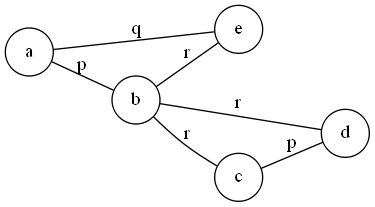
\includegraphics[width=.4\linewidth]{figure/apriori} 
					\label{fig:apriori_1}
			}}
			\quad 
			\subfloat[G2]{{
					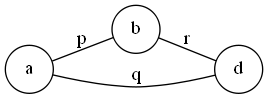
\includegraphics[width=.3\linewidth]{figure/apriori.2} 
					\label{fig:apriori_2}	
			}}
			\quad
			\subfloat[G3]{{
					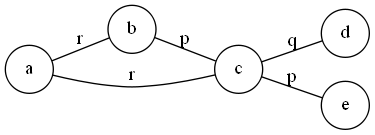
\includegraphics[width=.4\linewidth]{figure/apriori.3} 
					\label{fig:apriori_3}
			}}
			\quad 
			\subfloat[G4]{{
					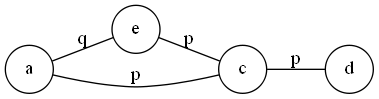
\includegraphics[width=.4\linewidth]{figure/apriori.4} 
					\label{fig:apriori_4}	
			}}
			\caption{Graph Dataset For Apriori-based Algorithm}
			\label{apriori}
		\end{figure}
	
		그림 \ref{apriori}는 Apriori-based Algorithm을 설명하기 위한 예시 그래프이다. 본격적으로 설명하기 전에 Minimum Support Count가 2임을 알린다.
	\newpage
		\begin{figure}[h]
			\centering
			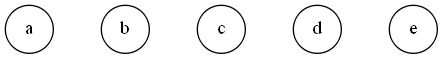
\includegraphics[width=.7\linewidth]{figure/apriori.5}
			\caption{k = 1 Frequent Subgraphs}
			\label{apriori_k_1}
		\end{figure}
	
		그림 \ref{apriori_k_1}은 k가 1일때 k-subgraph들을 나타낸다. 그림 \ref{apriori}의 그래프 G1, G2, G3, G4를 counting하면 a는 4번, b는 3번, c는 3번, d는4번, e는 3번이다. 그러므로 a,b,c,d,e 모두 조건을 만족하므로 Frequent Subgraph이다.
		
		\begin{figure}[h]
			\centering
			\subfloat[]{{
					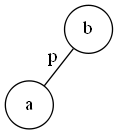
\includegraphics[width=.15\linewidth]{figure/apriori.6} 
					\label{fig:apriori_2_1}
			}}
			\quad 
			\subfloat[]{{
					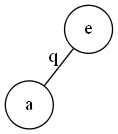
\includegraphics[width=.15\linewidth]{figure/apriori.7} 
					\label{fig:apriori_2_2}	
			}}
			\quad
			\subfloat[]{{
					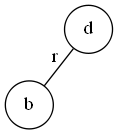
\includegraphics[width=.15\linewidth]{figure/apriori.8} 
					\label{fig:apriori_2_3}
			}}
			\quad 
			\subfloat[]{{
					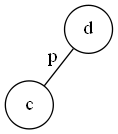
\includegraphics[width=.15\linewidth]{figure/apriori.9} 
					\label{fig:apriori_2_4}	
			}}
			\quad 
			\subfloat[]{{
					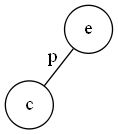
\includegraphics[width=.15\linewidth]{figure/apriori.10} 
					\label{fig:apriori_2_5}	
			}}
			\caption{k = 2 Frequent Subgraphs}
			\label{apriori_2}
		\end{figure}
		
		그림 \ref{apriori_2}는 k가 2일때 k-subgraph들을 나타낸다. 그림 \ref{apriori}의 그래프 G1, G2, G3, G4를 counting한 결과이다. 예를 들어 vertex a와 b로 이루어진 그래프 counting해 보자.
		
		
		\begin{figure}[h]
			\centering
			\subfloat[G1]{{
					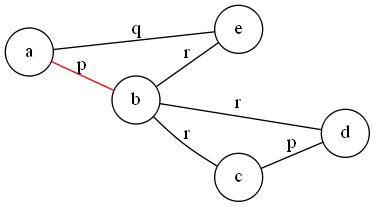
\includegraphics[width=.4\linewidth]{figure/G_example} 
					\label{fig:ex_1}
			}}
			\quad 
			\subfloat[G2]{{
					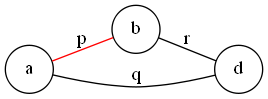
\includegraphics[width=.3\linewidth]{figure/G_example.2} 
					\label{fig:ex_2}	
			}}
			\quad
			\subfloat[G3]{{
					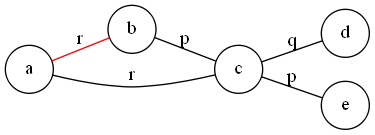
\includegraphics[width=.4\linewidth]{figure/G_example.3} 
					\label{fig:ex_3}
			}}
			\quad 
			\subfloat[G4]{{
					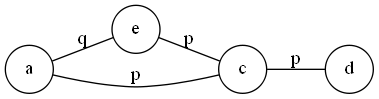
\includegraphics[width=.4\linewidth]{figure/G_example.4} 
					\label{fig:ex_4}	
			}}
			\caption{전체 dataset 중 vertex a와 b로 이루어진 edge 표시}
			\label{examples}
		\end{figure}
	
		\begin{enumerate}
			\item G1 (그림 \ref{fig:ex_1}) : vertex a와 b사이의 weight가 p
			\item G2 (그림 \ref{fig:ex_2}) : vertex a와 b사이의 weight가 p
			\item GE (그림 \ref{fig:ex_3}) : vertex a와 b사이의 weight가 r
		\end{enumerate}
		
		weight가 p인 것은 2개, r인 것은 1개로 p만 threshold를 만족한다. 이에 따라 vertex a와 b 사이의 weight가 p인 것(그림 \ref{fig:apriori_2_1})만이 Frequent Subgraph이다.
		
		\newpage
		
		\begin{figure}[h]
			\centering
			\subfloat[G1]{{
					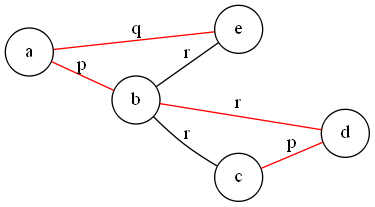
\includegraphics[width=.4\linewidth]{figure/ex} 
					\label{fig:ex1}
			}}
			\quad 
			\subfloat[G2]{{
					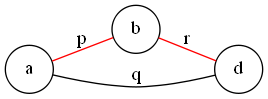
\includegraphics[width=.3\linewidth]{figure/ex.2} 
					\label{fig:ex2}	
			}}
			\quad
			\subfloat[G3]{{
					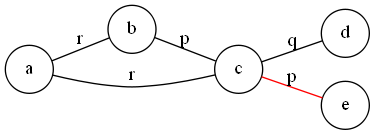
\includegraphics[width=.4\linewidth]{figure/ex.3} 
					\label{fig:ex3}
			}}
			\quad 
			\subfloat[G4]{{
					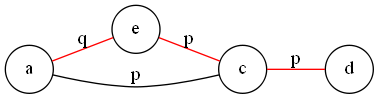
\includegraphics[width=.4\linewidth]{figure/ex.4} 
					\label{fig:ex4}	
			}}
			\caption{G1, G2, G3, G4에 k가 2인 Frequent Graph(그림 \ref{apriori_2} 참조)를 표시함}
			\label{ex} 
		\end{figure}
		
		그림 \ref{ex}를 참고해 k가 3인 Frequent Subgraph를 추출하면 그림 \ref{apriori_3}과 같다.

		
		\begin{figure}[h]
			\centering
			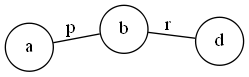
\includegraphics[width=.3\linewidth]{figure/apriori.11}
			\caption{k = 3 Frequent Subgraphs}
			\label{apriori_3}
		\end{figure}
		
		k=3일 때, Frequent Subgraph가 1개이므로 반복을 중단한다.
		
		

		\subsection{Pattern Growth approach}
			k개의 vertex 또는 edge를 가지는 subgraph 2개를 합쳐서 k+1개의 item들을 가지는 candidate를 만든다. 이 candidate는 threshold를 만족할 때 Frequent Subgraph가 된다.
			
			\subsubsection{Vertex Growing}
				\begin{figure}[h]
					\centering
					\subfloat[G1]{{
							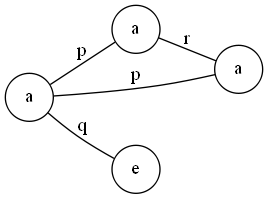
\includegraphics[width=.3\linewidth]{figure/vertex} 
							\label{vertex_1}
						}}
					\quad % tab : quad 1번 qquad 2번 => 얘 없으면 안됨
					\subfloat[G2]{{
							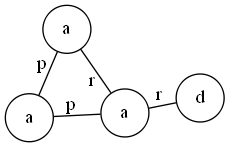
\includegraphics[width=.3\linewidth]{figure/vertex.2} 
							\label{vertex_2}	
						}}
					\caption{임의의 Graph G에 대한 subgraph}
					\label{vertex}
				\end{figure}
			
				위의 그림 \ref {vertex}는 임의의 그래프 G의 Subgraph이다. 이 때 이  Subgraph들은 threshold를 만족한다. 그림 \ref{vertex_1}와 그림 \ref{vertex_2}을 합쳐서 만든 새로운 candidate는 아래의 그림 \ref{vertex_3}와 같다.
				
			\newpage
				
				\begin{figure}[h]
					\centering
					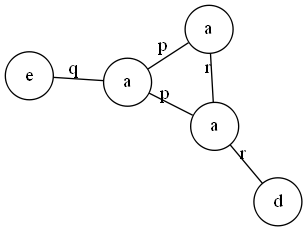
\includegraphics[width=.4\linewidth]{figure/vertex.3}
					\caption{G3 = join(G1,G2)}
					\label{vertex_3}
				\end{figure}
				
				
				그림 \ref{vertex_3}는 그림 \ref {vertex_1}에 vertex d, 그림 \ref {vertex_2}에 vertex e를 추가한 것과 같다. 이 candidate가 threshold를 만족하면 Frequent Subgraph가 된다.				
				
				그림 \ref {vertex_1}, 그림 \ref {vertex_2}, 그림 \ref {vertex_3}을 행렬으로 나타내보자.
				
				\begin{align}
					M_{G1} = 
					\begin{pmatrix}\label{M_G1}
						0 & p & p & q \\
						p & 0 & r & 0 \\
						p & r & 0 & 0 \\
						q & 0 & 0 & 0 \\
					\end{pmatrix}
					\\
					M_{G2} = 
					\begin{pmatrix}\label{M_G2}
						0 & p & p & q \\
						p & 0 & r & 0 \\
						p & r & 0 & 0 \\
						q & 0 & 0 & 0 \\
					\end{pmatrix}
				\end{align}
				
				식 (\ref{M_G1})은 그림 \ref{vertex_1}, 식 (\ref{M_G2})은 그림 \ref{vertex_2}에 각각 대응한다. 그림 \ref{vertex_1}와 그림 \ref{vertex_2}를 병합한 그림 \ref{vertex_3}에 대응하는 행렬은 아래와 같다.
				
				$$
				M_{G3} = 
				\begin{pmatrix}\label{M_G3}
					0 & p & p & 0 & q \\
					p & 0 & r & 0 & 0 \\
					p & r & 0 & r & 0 \\
					0 & 0 & r & 0 & 0 \\
					q & 0 & 0 & 0 & 0 \\
				\end{pmatrix}
				$$
			\newpage
			\subsubsection{Edge Growing}
				Edge Growing 또한 Vertex Growing과 유사하다. Vertex를 늘려가는 것이 아닌, Edge를 늘려가는 것 외에는 차이점이 없다.
				
				\begin{figure}[h]
					\centering
					\subfloat[G1]{{
							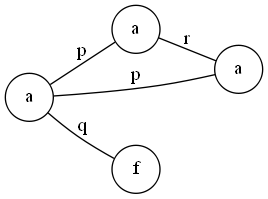
\includegraphics[width=.4\linewidth]{figure/edge} 
							\label{edge_1}
					}}
					\quad % tab : quad 1번 qquad 2번 => 얘 없으면 안됨
					\subfloat[G2]{{
							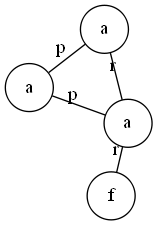
\includegraphics[width=.2\linewidth]{figure/edge.2} 
							\label{edge_2}	
					}}
					\caption{임의의 Graph G에 대한 subgraph}
					\label{edge}
				\end{figure}
			
				위의 그림 \ref {edge}은 임의의 그래프 G에 대한 subgraph G1, G2이다. 이 때 이  Subgraph들은 threshold를 만족한다. 이 두개의 subgraph를 병합해 만든 candidate는 그림 \ref {edge_3}과 같다. 이 candidate가 threshold를 만족하면 Frequent Subgraph가 된다.
				
				\begin{figure}[h]
					\centering
					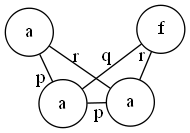
\includegraphics[width=.3\linewidth]{figure/edge.3}
					\caption{G3 = join(G1,G2)}
					\label{edge_3}
				\end{figure}
	\section{Result}
		Frequent Subgraph를 찾는 2가지 방법을 살펴보았다. 두 방법 모두 좋은 방법이지만 단점도 존재한다.	Apriori-based와 같은 경우 n개의 edge가 존재한다고 가정했을때, $2^n$개의 Subgraph가 발생한다. 이러한 단점을 극복한 방법을 적절히 사용한다면, 효율적으로 Frequent Subgraph를 찾을 수 있을것이다.
	
\end{document}
